\section{zadanie 6}

\subsection{Wyniki:}
Zadanie polegało na przetestowaniu funkcji /(rysujNnfx/) przygotowanej na potrzeby wcześniejszego zadania. Testy zostały wykonane na następujących danych wejściowych:
\begin{enumerate}
  \item \(f(x) = |x|; [a, b] = [-1, 1], n = 5, 10, 15 \)
  \item \(f(x) = \frac{1}{1 + x^2}; [a, b] = [-5, 5], n = 5, 10, 15 \)
\end{enumerate}

\begin{figure}[t]
  \centering
  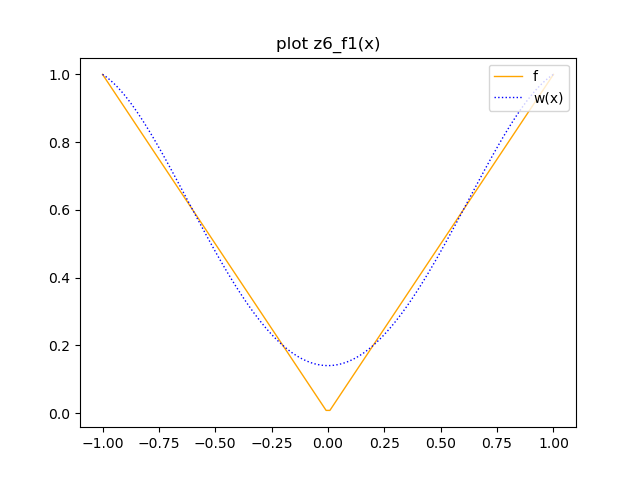
\includegraphics[width=\textwidth]{plot_z6_f1(x)_5.png}
  \caption{Wykres funkcji \(f(x) = |x|, n = 5\)}
\end{figure}

\begin{figure}[t]
  \centering
  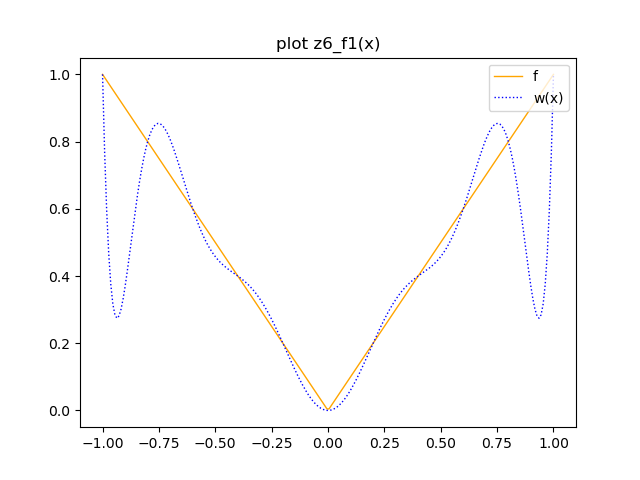
\includegraphics[width=\textwidth]{plot_z6_f1(x)_10.png}
  \caption{Wykres funkcji \(f(x) = |x|, n = 10\)}
\end{figure}

\begin{figure}[t]
  \centering
  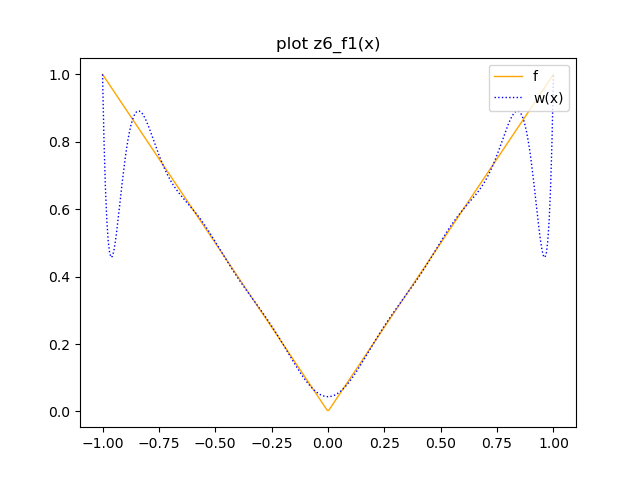
\includegraphics[width=\textwidth]{plot_z6_f1(x)_15.png}
  \caption{Wykres funkcji \(f(x) = |x|, n = 15\)}
\end{figure}

\begin{figure}[t]
  \centering
  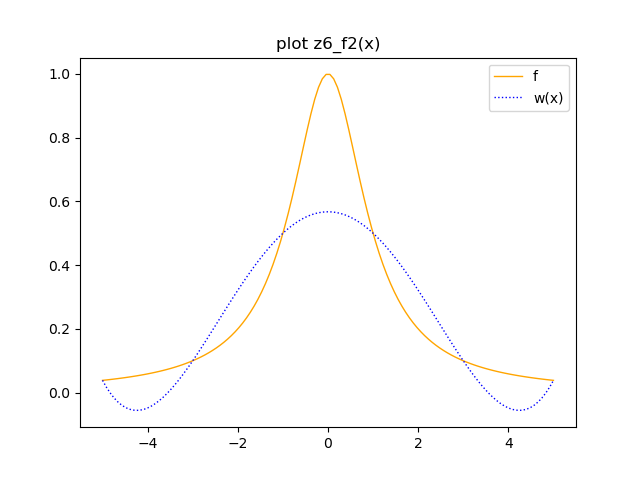
\includegraphics[width=\textwidth]{plot_z6_f2(x)_5.png}
  \caption{Wykres funkcji \(f(x) = \frac{1}{1+x^2}, n = 5\)}
\end{figure}

\begin{figure}[t]
  \centering
  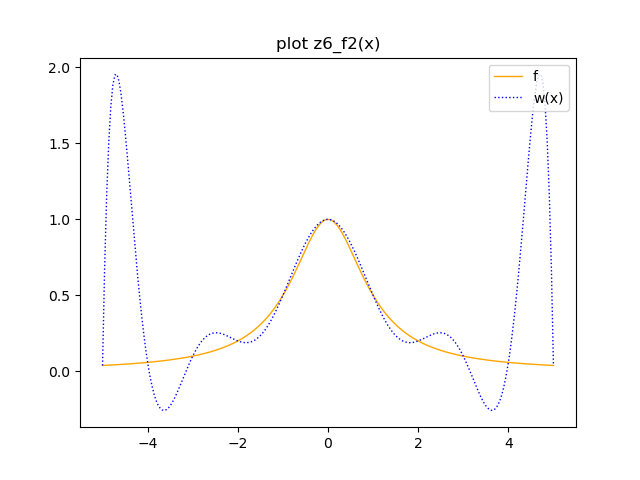
\includegraphics[width=\textwidth]{plot_z6_f2(x)_10.png}
  \caption{Wykres funkcji \(f(x) = \frac{1}{1+x^2}, n = 10\)}
\end{figure}

\begin{figure}[t]
  \centering
  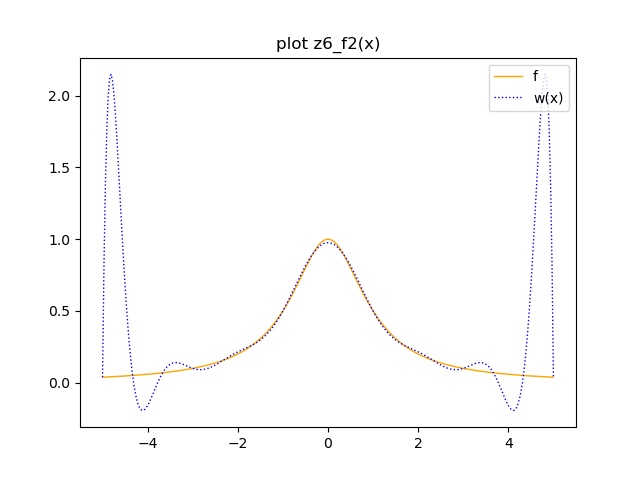
\includegraphics[width=\textwidth]{plot_z6_f2(x)_15.png}
  \caption{Wykres funkcji \(f(x) = \frac{1}{1+x^2}, n = 15\)}
\end{figure}

\subsection{Wnioski:}
Dla testowanych funkcji przybliżenia niezbyt wiernie oddają spodziewane kształty.
W tych przypadkach możemy zaobserwować efekt Rungego. Jest to zjawisko polegające na pogorszeniu się jakości interpolacji mimo zwiąkszenia liczby jej węzłów co jest efektem odwrotnym do zamierzonego. Efekt jest wywołany przez równomierne rozłożenie węzłów interpolacji. Można go uniknąć kładąc więcej węzłów interpolacji na końcach przedziału.
